%\section{Opportunities of spatial and temporal correlation}
\section{Key ideas in {\name}}
\label{sec:insights}

Naive continuous profiling is expensive for three main reasons. We have to profile all the video from a video stream, we have to profile all video streams in the system, and finally, the configuration space is exponentially large.
\name tackles these challenges using the following domain-specific, empirical observations about the impact of configurations on the accuracy and cost of video analytics pipelines.
First, if the underlying characteristics of the video that affect the configurations' resource-accuracy tradeoffs persist over time, we can learn these {\em temporal correlations} to reuse configurations over time. 
Second, if two video feeds share similar characteristics, it is likely they will also share the same configurations. Such {\em cross-camera correlations} open up opportunities to significantly reduce the profiling cost by amortizing this cost across many camera feeds. % and over time.
Finally, we have experimentally observed that many of the configuration knobs {\em independently} impact accuracy. This allows us to dramatically reduce the search space. Next, we provide the intuition behind these three key observations, and discuss the implications on the design of {\name} (\S\ref{sec:algorithm}).

\comment{
To reduce the profiling cost 
%while still improving accuracy and resource
%consumption, \name leverages 
%the domain-specific insight that the performance of \nn configurations show substantial {\em spatial and temporal correlation}.
\name leverages domain-specific empirical observations about the configurations of video analytics pipelines. 
%That is, if some underlying characteristics that affect configurations' resource-accuracy tradeoffs persist over the duration of a video feed, the optimal \nn configuration might tend to persist too.
}

\subsection{Persistent characteristics over time}
\label{subsec:temporal}

While the characteristics of videos change over time, there are opportunities to learn the performance provided by different configurations, both good and bad. This is because the underlying characteristics of the video objects (\eg size, class, angle) that affect the accuracy tend to remain relatively stable over time. 

As a result, configurations that are particularly bad tend to remain so. For example, if a camera is covering objects from the side-view and an object detector is not tuned to detect objects at a side-view angle, it will almost always produce results with low accuracy, and hence it should not be selected. Such configurations can be learned and discarded from the profiling for longer periods of time. 

Similarly, good configurations also tend to consistently produce good performance. A common example is surveillance video, which tends to have  static content. For such videos, a low-cost configuration (\eg low frame rate) would be sufficient for a long period of time. More generally, although the best configuration, \ie the one with the lowest  cost meeting the accuracy threshold $\alpha$, might change frequently, the set of {\em top-$k$ best configurations} (top-$k$ cheapest configurations with accuracy $\geq \alpha$) tend to remain stable over time. Thus, we can dramatically reduce the search space by restricting ourselves to these top-$k$ configurations.
%to find the best configuration, we can learn and restrict the profiling to this stable set of top-K configurations. 
%\ga{Can we add a graph in support of the top-K point?}

Neither of these rules holds all of the time. Thus, it is crucial that we periodically explore the full configuration space, to give previously bad configurations the opportunity to prove their worth, and allow previously good configurations to fall from grace. 

%\ga{OLD TEXT in rest of 4.1; Junchen \& Sid to revise/delete.}

\comment{
Furthermore, although the performance of video analytics pipelines varies over time, we often observe relative long time intervals for which the performance doesn't change. One scenario is when the video content is static, as it is often the case for surveillance cameras. In this scenario, a low-cost configuration (e.g., low frame rate) could be sufficient for a long time. Even when the video content is dynamic, some of the video characteristics can persist over time, which means that the same \nn configuration can have relatively stable accuracy over the same time period.  Such underlying characteristics include the size of the objects, their speeds, object classes likely to appear, all of which bear significant impact on the value of best configurations.
}

% \Figure~\ref{??} shows a particular configuration on a given video feed over time. As annotated, 
Indeed, factors like object size and velocity,
which affect the inference accuracy, do not change at a dramatic rate. To show the distribution of the time intervals over which the video characteristics remain relatively the same, we define the persistence of a configuration $c$ as the length of continuous frames which $c$'s accuracy {\em exceeds a threshold $\alpha$ for over 95\% of frames}\footnote{We do not use 100\% to prevent noise.}. Figure~\ref{fig:persistence} shows the distribution of the persistence for two typical configurations. We observe that half of the times, the configurations persistently exceed the accuracy threshold for more than 200 frames (roughly 6 seconds of video with 30fps).
The spatial similarity of cameras manifested in similarities between their resource-accuracy profiles. For instance in Figure~\ref{fig:cross-camera}, by varying frame rate, Camera \#1 and Camera \#2 in Figure~\ref{fig:similar cameras} share similar resource-accuracy profile, and is different to that a third camera.

\begin{figure}
    \centering
    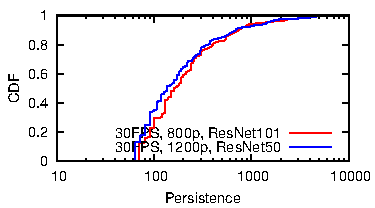
\includegraphics[width=0.35\textwidth]{PaperGraphs/PersistenceCDF.pdf}
    \caption{Distribution of persistence of two typical configurations. }
    \label{fig:persistence}
\end{figure}


\subsection{Cross-camera similarities}
\label{subsec:spatial}

Even when cameras do not observe the same scene, 
%have an overlap in the scene they are covering (so the video content has little in common), 
their video feeds can still share similar characteristics. For instance, the videos from a set of surveillance cameras covering an enterprise building will likely share similar classes of objects, lighting, viewing angles, and so on. 
%All of these characteristics have significant impact on the resource-accuracy tradeoffs.
Such similarity can also occur for traffic cameras deployed in a city.
Figure~\ref{fig:similar cameras} shows two such similar cameras.
The vehicles in the city will likely have similar moving speeds, lighting that is influenced by weather conditions, and viewing angles due to the cameras being installed at similar heights (as a result of  uniform installation policies). Even if the cameras are not in geographic proximity, cameras deployed for the same purpose such as traffic analytics are likely to exhibit similarities. This can happen due to the underlying similarity of street planning, say, across a country. 

\begin{figure}
    \centering
    \hspace{-0.5cm}
    \subfloat[Camera \#1]
    {
        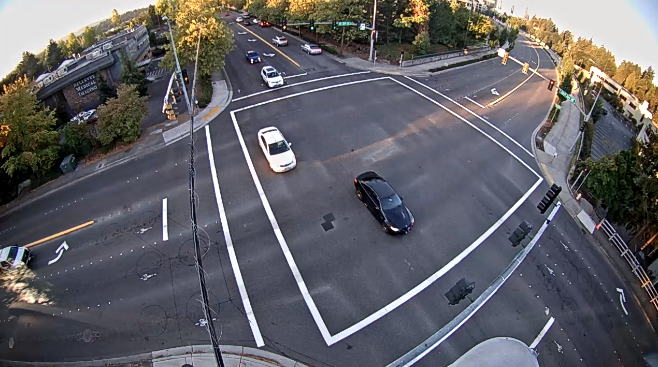
\includegraphics[width=0.22\textwidth]{PaperGraphs/Screenshot1.png}
    }
    \subfloat[Camera \#2]
    {
        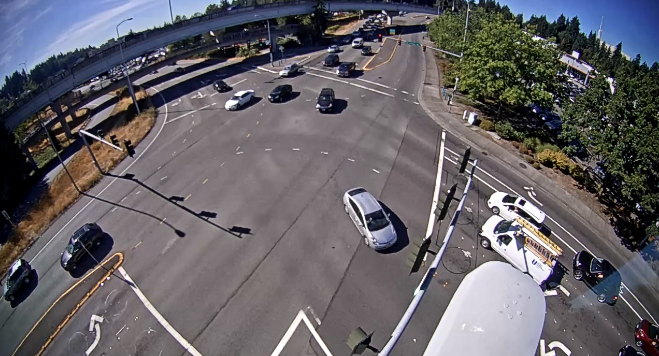
\includegraphics[width=0.22\textwidth]{PaperGraphs/Screenshot2.png}
    }
    \caption{Screenshots of two similar cameras.}
    \label{fig:similar cameras}
\end{figure}

%is reason to believe that video feeds from cameras in 
%close vicinity often have similar characteristics that affects 
%video analytics performance, and hence
%they will have similarity in their best configurations.
%For instance, cameras in the same city all have simiar
%objects moving speed, type of objects, lighting, camera 
%angle and height, and weather conditions, all of which have
%significant impact on the accuracy-resource tradeoffs.

% As we hinted before, the relationship between configurations 
% and the resulting inference accuracy depends on several high-level 
% characteristics other than the content itself, and these 
% characteristics are much more likely to resemble across multiple 
% video feeds. 
% For instance, if two video feeds contain objects moving at similar
% speeds, they will likely to share the same ideal frame rate. 

%Video feeds sharing key characteristics are abundant in practice. 
% Traffic videos in close vicinity often show vehicles appear at 
% similar speeds, in similar size, and with similar 
% brightness/contrast, all of which have significant impact on the 
% accuracy-resource tradeoffs.
%In fact, such spatial correlations can be found in most types of surveillance videos.
Video feeds that exhibit these kinds of spatial correlations are abundant in practice, especially in real-time applications such as traffic monitoring and building surveillance, where many cameras provide similar video feeds. 
%More importantly, in a system for real-time video analytics, these similar video feeds are often available %en masse  from many cameras {\em simultaneously}. 
This offers a great opportunity to reduce profiling cost by amortizing this cost over many similar video feeds.

Note that the spatial correlations of best configurations does not mean that applying the same configuration will produce the exact same accuracy on different videos. The timescales at which such correlation emerges can be larger than the timescale at which the accuracy changes. Thus, we should not blindly reuse the best configuration on another video, even when the characteristics of the two videos are deemed very similar. Instead, we can leverage the fact that similar videos tend to have similar {\em distributions} of best configurations. Then, we can use the most promising configurations from one camera---\eg the top-$k$ best configurations---to guide the search for a spatially-related camera. 
%\ga{The above paragraph is unclear in what it's leading to...}
% Figure~\ref{??} shows real-world examples where video feeds with
% similar share almost identical resource-accuracy
% tradeoffs of certain knobs, and therefore, their best 
% configurations.

% \jc{insert the figures here.}

\begin{figure}
    \centering
    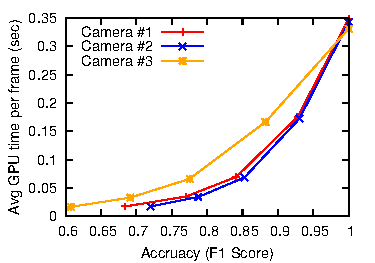
\includegraphics[width=0.3\textwidth]{PaperGraphs/CrossCamera_profiles.pdf}
    \caption{The spatial similarity of cameras manifested in similarities between their resource-accuracy profile: By varying frame rate, Camera \#1 and Camera \#2 share similar resource-accuracy profile, and is different to that Camera \#3.}
    \label{fig:cross-camera}
\end{figure}


\subsection{Independence of configuration knobs}
\label{subsec:independence}

% PETER
%To further simplify the search in the exponentially-large configuration space, we observe that, typically, the individual knobs have \emph{independent} impact on accuracy. For example, consider a pipeline with the resolution and frame rate knobs, with values $(480p,720p,960p)$ and $(1, 10, 30)$, respectively. We assume that the reduction in accuracy from the golden config $(960p,30)$ to $(720p,30)$ is similar to reduction in accuracy from $(960p,10)$ to $(720p,10)$. This approximation lets us prune large parts of the configuration space and estimate accuracy of configurations even without profiling them.

%In additional significant cost, even when profiling a \emph{cheap} configuration $c$, is the requirement to execute the golden configuration (which is very expensive) on the same dataset to provide the ground truth for computing accuracy of $c$. Instead, we can implement the following optimization; first identify a \emph{proxy golden configuration} $c^*_p$, which is much cheaper than the golden configuration, but is still very accurate and then use $c^*_p$ to generate ground truth data for evaluating any other configurations.

%Our second observation is that the knobs have monotonic impact on configuration cost. Specifically, the values of each knob can be ordered such that increasing the value of a knob (while holding the other knobs fixed), increases the resource demand of the configuration. For example, increasing frame rate results in higher cost since we have to process more pixels, independent of the image resolution and object detection model.

% GANESH
To further simplify the search in the exponentially-large configuration space, we observe that, typically, the individual knobs have \emph{independent} impact on accuracy. For example, consider a pipeline with the resolution and frame rate knobs, with values (480p,720p,960p) and (1, 10, 30), respectively. Recall from \S\ref{sec:potential} that we measure the accuracy (F1 score) of configurations relative to a golden configuration, which in this case is (960p, 30).  We observe empirically that in most cases the accuracy of configuration (480p, 30) relative to (960p, 30) {\em is similar in value to} the accuracy of (480p, 10) relative to (960p, 10). %We assume that the reduction in accuracy from the golden configuration (960p,30) to (720p,30) {\em is similar to} the reduction in accuracy from (960p,10) to (720p,10).  

This has two important implications.  First, it lets us tune the resolution knob {\em independent} of the frame rate; this prunes a large part of the configuration space. Second, it lets us estimate a configuration's accuracy by combining its per-knob accuracies; in particular, we can do this {\em without} running the expensive golden configuration. 

%To further simplify the search in the exponentially-large configuration space, we observe that, typically, the individual knobs have \emph{independent} impact on accuracy. Recall from \S\ref{sec:potential} that we measure the accuracy of configurations relative to a golden configuration. For example, consider a pipeline with the resolution and frame rate knobs, with values (480p, 720p, 960p) and (1, 10, 30), respectively. The golden configuration is using (960p, 30). 

%As per the observation on independence of knobs, the accuracy of configuration (480p, 30) relative to (960p, 30) {\em is similar in value to} the accuracy of (480p, 10) relative to (960p, 10). This has two important implications. First, we can vary the resolution knob {\em independent} of the value of the frame rate. This lets us prune large parts of the configuration space during profiling. Second, we can estimate the accuracy of configurations {\em without} running the expensive golden configuration. 

Further, the {\em relative ordering} between the configurations on their resource demand will be unaltered between using frame rates 30 and 10. That is, if the resource demand of (480p, 30) is less than that of (720p, 30), then this ordering will continue be true with the resource demand of (480p, 10) being less than (720p, 10). In our setting, the configuration knobs have {\em monotonic} impact on cost, \ie increasing the value of a knob while holding the other knobs fixed increases the resource demand of the configuration.

%Our second observation is that the knobs have monotonic impact on configuration cost. Specifically, the values of each knob can be ordered such that increasing the value of a knob (while holding the other knobs fixed), increases the resource demand of the configuration. For example, increasing frame rate results in higher cost since we have to process more pixels, independent of the image resolution and object detection model.


% COMMON
Since our objective is to pick the cheapest configuration that meets the desired accuracy threshold, the above observations allow us to significantly reduce the profiling costs.

An important note to keep in mind is that the accuracy of these observations is not crucial to our solution. Indeed, assume for the sake of the argument that these observations are not entirely accurate. Then, if one were to account for these inaccuracies, it would only improve our solution. Thus, subject to these observations, our solution can be seen as a lower bound, which can be further improved by refining these observations. We leave such refinements for future work.

\comment{
If we reduce the resolution from 960p to 720p, we assume that the relative impact on accuracy (e.g., reduction by 20\%) is independent of the values of the frame rate knob.
}

\comment{
In particular, we observe that the impact of 
these knobs on accuracy is determined by {\em orthogonal} factors. 
For instance, in pipeline $A$, the frame rate is influenced by the object
moving speed, image size affects the number of pixels that cover 
each object of interest, and the object detection model depends on 
whether the shape of an object can be expressed by the extracted 
features. This allows us to make deductions like: if 5fps is the lowest
frame rate that achieves an F1 score of 0.8 when the image size is 480p, 
then 5fps will be the lowest frame rate to attain an F1 score of 0.8 when the image size 
is 960p.}

\comment{
To further simplify the search in the exponentially-large configuration space, we observe, that typically the individual knobs have \emph{independent} (multiplicative) and monotonic impact on accuracy. 
Let $v_{r,i}$ be the $i^{\text{th}}$ value of knob $r$. For configuration $c = (v_{1,i_1}, \dots, v_{n,i_n})$, we can approximate its accuracy as follows $A(c) = \prod_{r} L_{r,i_r}$, where $L_{r,i_r}$ is the relative impact on accuracy of knob $r$ when using value $i_r$. 
For example, consider the frame rate and image size knobs with values $(1,10,30)$ and $(480p,720p,960p)$, respectively. For higher frame rates and image sizes, we expect higher accuracy since we do not skip frames and can detect smaller objects. We can encode this using $L$ vectors such as $(0.1, 0.5, 1)$ and $(0.6, 0.8, 1)$. Using this, we can approximate accuracy of a sample configuration $(10,720p)$ as $0.5 \cdot 0.8 = 0.4$.

This is a crucial observation because it allows us to reduce the profiling cost of both the golden configuration (which is very expensive, \S\ref{subsec:profiling-cost}) as well as other configurations.
}

\comment{
While just an approximation, as we demonstrate in our evaluation, this observation lets us efficiently navigate the configuration space and find accurate and cheap configurations.
}


\comment{
A helpful empirical observation we make is regarding the {\em independence} of the knobs of the configurations. To illustrate this independence we use a simple example. Consider the previous pipeline characterized by just two knobs: frame resolution ($r$)  and object detection model ($d$). Let $\langle r*, d* \rangle$ be the values of these two knobs for the golden configuration. As per the independence observation, two aspects hold. 

First, the relative accuracy of a configuration, $\langle r_i, d*\rangle$, where $r_i$ is a resolution lower than its golden value, compared to the golden configuration, $\langle r*, d*\rangle$, {\em is similar to} the relative accuracy of $\langle r_i, d_i\rangle$ against $\langle r*, d_i\rangle$. This means that if the available resolutions are 480p, 720p, 960p (golden value), and the available models are tiny Yolo and full Yolo (golden), we can profile the resolutions by varying them using just the tiny Yolo model instead of using the expensive full Yolo. In other words, the impact on the accuracy of resolution is {\em independent} of the detection model. \ga{We need an intuition.}
}

\comment{
Further, while the absolute resource consumption of the configurations without using the golden values will be different, the {\em relative ordering} between the configurations (resolutions) on their resource consumption will be unaltered between using the tiny or full Yolo models. In other words, if the resource consumption of $\langle r_i, d* \rangle$ is greater than the resource consumption of $\langle r_j, d* \rangle$, then the resource consumption of  $\langle r_i, d_k \rangle$ will be greater than the resource consumption of $\langle r_j, d_k \rangle$, for any $d_k$. \ga{Example.}
}